\documentclass[a4paper]{article}
\usepackage{graphicx}
\parindent=0em
\begin{document}
Q1.\\
i.\\
ACEF, BCEF are candidate keys.\\
$AD\rightarrow B$: AD does not contain a key. $C\rightarrow D$: C does not contain a key. $BC\rightarrow A$: BC does not contain a key. $B\rightarrow D$: B does not contain a key.\\\\
Decomposition:\\
Based on the functional dependency $AD\rightarrow B$, decompose ABCDEF into relations ACDEF, ADB;\\
Based on the functional dependency $C\rightarrow D$ , decompose ACDEF into relations ACEF, CD;\\\\
Taken together, decompose ABCDEF into relations ACEF, CD, ABD.\\
\\ii.\\
AF, CF are candidate keys.\\
$BC\rightarrow E$: BC does not contain a key. $C\rightarrow AB$: C does not contain a key.\\\\
Decomposition:\\
Based on the functional dependency $C\rightarrow AB$, decompose ABCDEF into relations CDEF, ABC. This is in BCNF.\\
\\iii.\\
ABCF, BCDF are candidate keys.\\
$ABF\rightarrow D$: ABF does not contain a key. $CD\rightarrow E$: CD does not contain a key. $BD\rightarrow A$: BD does not contain a key.\\\\
Decomposition:\\
Based on the functional dependency $ABF\rightarrow D$, decompose ABCDEF into relations ABCEF, ABFD.\\
Based on the functional dependency $BD\rightarrow A$, decompose ABFD into relations BDF, ABD.\\\\
Taken together, decompose ABCDEF into relations ABCEF, BDF, ABD.\\
\\iv\\
AB is the candidate key.\\
$BCD\rightarrow EF$: BCD does not contain a key. $B\rightarrow C$: B does not contain a key.\\ \\
Decomposition:\\
Based on the functional dependency $B\rightarrow C$, decompose ABCDEF into relations ABDEF, BC. This is in BCNF.\\

\par
Q2.\\
\\Symbol legends:\\
$\pi:\ Projection$\\
$\sigma:\ Selection$\\
$\rho:\ Rename$\\
$\gamma:\ Aggregation\ (GroupBy)$\\
$\bowtie:\ Join$\\
$R: Relation$\\
$Res: Result$\\
\\
i.\\
$Res\ =\ \pi _{name}(\sigma_{sector\ =\ 'Technology'}(Company\ \bowtie\ Category))$\\
\\ii.\\
$Res\ =\ \pi _{code}(\sigma_{personCount\ >\ 5}(\rho _{code,personCount}(\gamma _{code, count(Person)}(Executive)))  $\\
\\iii\\
$Res\ =\ \pi _{person}(\sigma _{companyCount\ >\ 1}(\rho _{person, companyCount} ( \gamma _{person, count(Code)}(Executive)))) $\\
\\iv\\
$R(industry)\ =\  \pi _{industry}(\sigma _{compantCount\ =\ 1}(\rho _{industry, companyCount}(\gamma _{industry, count(Code)}(Category)))$\\
$Res\ =\ \pi _{code, industry}(Category\ \bowtie \ R(industry))$\\
\par
Q3.\\
i.\\
$R\ \cup \ (S\ \cap \ T)$, has:\\
minimal r, maximal r + min(s, t) tuples.\\
\\ii\\
$\sigma _{c}(R\ \times \ S)$ for some condition c, has:\\
minimal 0, maximal r*s tuples.\\
\\iii\\
$R\ -\ \pi _{a}(R\  \bowtie \ S)$ for some list of attributes a, has:\\
minimal 0, maximal r tupples.\\
\par
Q4\\
i.\\\\
\begin{tabular}{lllllllll}
T1: & R(x) &      & W(x) &      & R(y) &      & W(y) &      \\ 
T2: &      & R(x) &      & W(x) &      & R(y) &      & W(x)
\end{tabular}% 
\\\\
T2:R(x), T1:W(x) gives conflict $T2 \rightarrow T1$;\\
T1:W(x), T2(W(x) gives conflict $T1 \rightarrow T2$;\\
T2:R(y), T1W(y) gives conflict $T2 \rightarrow T1$.\\
This is not serializable due to multiple cycles, depicted as below:
\\ 
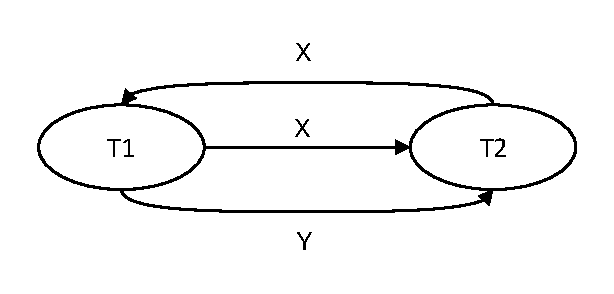
\includegraphics[scale=1]{fig1.pdf}
\\\\ii.\\\\
\begin{tabular}{lllllllll}
T1: &      &      &     & W(y) &      &      &      & R(x) \\ 
T2: &      &      &     &      & R(y) &      & W(x) &      \\ 
T3: & R(x) &    &       &      &      & R(d) &      &      \\ 
T4: &      & W(y) & W(z) &      &      &      &      &     
\end{tabular}
\\\\
T3:R(x), T2:W(x) gives conflict $T3 \rightarrow T2$;\\
T4:W(y), T1:W(y) gives conflict $T4\rightarrow T1$;\\
T1:W(y), T2:R(y) gives conflict $T1\rightarrow T2$;\\
T2:W(x), T1:R(x) gives conflict $T2\rightarrow T1$.\\
This is not serializable due to a cycle, depicted as below:\\ 
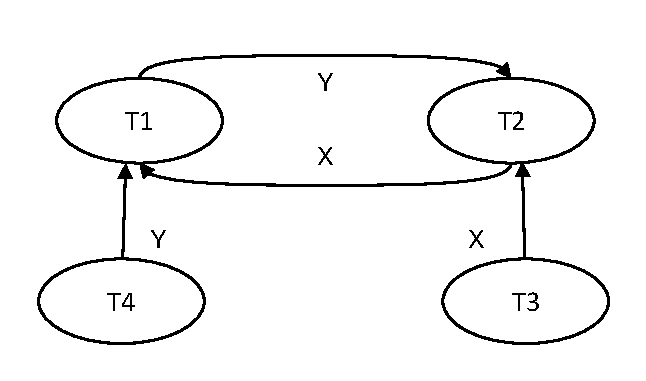
\includegraphics[scale=1]{fig2.pdf}
\end {document}



















